\documentclass{article}

\usepackage[dblblindworkshop]{neurips_2026}
\workshoptitle{Economics for Machine Learning}

\usepackage[utf8]{inputenc}
\usepackage[T1]{fontenc}
\usepackage{hyperref}
\usepackage{url}
\usepackage{booktabs}
\usepackage{amsfonts}
\usepackage{amsmath}
\usepackage{nicefrac}
\usepackage{microtype}
\usepackage{graphicx}
\usepackage{caption}
\usepackage{subcaption}
\usepackage{xcolor}

\captionsetup{font=small,labelfont=bf}

% ---- quantities reported in the text, taken from results.json ----
\newcommand{\Ncat}{868}
\newcommand{\Nactive}{457}
\newcommand{\Nopen}{175}
\newcommand{\Nscored}{180}
\newcommand{\CovScored}{91}
\newcommand{\OpenTok}{68}
\newcommand{\OpenSpend}{30}
\newcommand{\HHItok}{1183}
\newcommand{\HHIspend}{2439}
\newcommand{\PCone}{98}
\newcommand{\PCfive}{91}
\newcommand{\LagDays}{105}
\newcommand{\PriceRatio}{1.4}
\newcommand{\HostsOpen}{14.9}
\newcommand{\HostsClosed}{3.0}
\newcommand{\ChangeRate}{2.9}
\newcommand{\NeverRepriced}{54}
\newcommand{\MonthlyFreq}{12.6}
\newcommand{\PriceDuration}{7.4}
\newcommand{\CutShare}{58}
\newcommand{\SurvSix}{56}
\newcommand{\SurvTwelve}{45}
\newcommand{\PanelObs}{19{,}803}
\newcommand{\PanelModels}{634}
\newcommand{\PanelStart}{November 2023}
\newcommand{\PanelEnd}{May 2026}
\newcommand{\NRevisions}{708}
\newcommand{\NPriceEvents}{306}
\newcommand{\ElastTok}{$-0.53$}
\newcommand{\ElastTokSE}{0.10}
\newcommand{\ElastReq}{$-0.46$}
\newcommand{\ElastReqSE}{0.09}
\newcommand{\ElastCross}{$-0.24$}
\newcommand{\NEvents}{10}
\newcommand{\NEventsOpen}{5}
\newcommand{\MarketGrowth}{65}
\newcommand{\EntrantShare}{28}
\newcommand{\IncumbentGrowth}{18}
\newcommand{\EntryGrowthShare}{72}
\newcommand{\DiversionMDE}{0.13}
\newcommand{\CFmodels}{172}
\newcommand{\CFprice}{156}
\newcommand{\CFcs}{21}
\newcommand{\CFdollars}{2.4}
\newcommand{\CFhhiBase}{897}
\newcommand{\CFhhiCf}{1048}
\newcommand{\TaskCFprice}{18}
\newcommand{\TaskCFcs}{13}
\newcommand{\Ntasks}{29}
\newcommand{\MatchedRatio}{3.3}
\newcommand{\MatchedWeighted}{1.7}
\newcommand{\RealisedOpen}{0.35}
\newcommand{\RealisedClosed}{1.95}
\newcommand{\EntrantOpen}{69}
\newcommand{\OpenShareEarly}{86}
\newcommand{\OpenShareTrough}{29}
\newcommand{\OpenShareLate}{48}
\newcommand{\CFoutside}{2.4}
\newcommand{\NMajor}{19}
\newcommand{\IncGrowthLong}{0.25}
\newcommand{\IncDeclineShare}{32}
\newcommand{\MktGrowthLong}{0.52}

\title{Entry Without Displacement:\\How Open-Weight Models Compete in the Market for Inference}

\author{Anonymous}

\begin{document}

\maketitle

\begin{abstract}
Open-weight models are widely expected to constrain the pricing power of proprietary
model providers, but the mechanism has not been measured. We assemble a market-wide
panel of the models served by a large inference router: posted prices, capability
benchmarks, weight-release status and revealed usage for \Nactive{} models, extended
back to 2023 with archived catalogues. Three facts emerge. Competition works through
releases rather than repricing: \NeverRepriced\% of models are never repriced at all,
and a posted price changes in only \MonthlyFreq\% of model-months, even though changing
it costs a provider nothing. When prices do change, volume responds weakly, with an
own-price elasticity of \ElastTok{} (s.e.\ \ElastTokSE) identified from \NRevisions{}
revisions with model and date fixed effects. Entry does not displace incumbents:
over four weeks, models released inside the window took \EntrantShare\% of tokens
while incumbent volume grew \IncumbentGrowth\%, and the confidence interval rules out
differential losses above \DiversionMDE{} log points for the incumbents closest to an
entrant in capability space. Removing open-weight models from the choice set in an estimated
nested-logit demand system raises the average price paid per token by \CFprice\% and
costs users about \$\CFdollars{}m per day on this platform, while raising provider
concentration. Open weights discipline the price at which new demand is served, not
the prices incumbents post.
\end{abstract}

\section{Introduction}

Whether open-weight models constrain the market power of proprietary model providers
is now a policy question as much as an economic one. Reports commissioned by
governments name it as an open evidence gap \citep{bengio2026}, and the theoretical
case cuts both ways: scale economies in training push toward concentration
\citep{korinek2025}, while freely downloadable weights supply a competitive fringe
that any hosting provider can serve. Recent empirical work has begun to describe the
market. \citet{demirer2025} document a collapse in the price of a unit of measured
intelligence and a proliferation of suppliers; \citet{nagle2025} show that a large
share of proprietary usage is directed at models that are dominated on price and
measured capability by an open alternative, and estimate the savings foregone.

Both of those results are about the allocation of demand across models at a point in
time. Neither identifies the channel through which open weights would constrain
proprietary pricing, and the two natural channels have opposite implications for
policy. If open weights force incumbents to cut posted prices, then the constraint is
visible in the price series of established models and its strength can be read off
their price responses. If instead open weights capture new demand while incumbents
hold their prices, the constraint operates on the terms at which the market grows,
and any measurement based on incumbent price responses will find nothing.

We assemble a panel that can separate the two. Our data come from a large inference
router that publishes model-level usage, prices and capability scores. We combine the
current cross-section (\Nactive{} models with observed usage, \Nopen{} of them
open-weight), a daily usage panel covering all of them for one month, task-level
market shares for \Ntasks{} distinct uses, per-provider hosting terms, and a panel of
archived price catalogues and usage leaderboards reaching back to 2023. The panel
used for price responses contains \PanelObs{} model-date observations on
\PanelModels{} models.

Three facts follow, and they point the same way. First, the posted price of a given
model version behaves like a fixed characteristic of the product: \NeverRepriced\% of
models are never repriced, and the monthly frequency of a price change is
\MonthlyFreq\%, comparable to consumer goods \citep{nakamura2008,cavallo2018} in a
setting where the menu cost that explains rigidity there does not exist. Second, when prices do change, volume moves little.
Exploiting \NRevisions{} revisions with model and date fixed effects, we estimate an
own-price elasticity of \ElastTok{} (s.e.\ \ElastTokSE), below the value near one
reported by \citet{demirer2025} from cross-model variation and far below what
homogeneous-goods reasoning would imply. Third, entry is absorbed by growth rather
than by displacement. Over the four weeks of the daily panel the market grew
\MarketGrowth\%; models released inside the window took \EntrantShare\% of tokens,
of which \NEventsOpen{} of \NEvents{} releases were open-weight, and yet incumbent
volume rose \IncumbentGrowth\%. In an incumbent-by-entrant event study we find no
differential decline for the incumbents technologically closest to an entrant, with a
confidence interval that excludes declines larger than \DiversionMDE{} log points.

Read together, these facts say that the competitive constraint from open weights does
not show up where one would look for it. We therefore quantify it where it does show
up. We estimate a nested-logit demand system over the \CFmodels{} models with prices
and capability scores, invert it to recover mean utilities that reproduce observed
shares, and delete open-weight models from the choice set. Users would pay \CFprice\%
more per token, and the surplus loss is worth about \$\CFdollars{}m per day on this
platform alone. The loss is not evenly spread: across \Ntasks{} task-level markets,
the implied price increase rises almost one for one with the open-weight share of
task spending, from \TaskCFprice\% on average to more than twice that in agentic and
coding work. Concentration moves the other way from the usual presumption: removing
open weights raises the provider Herfindahl index from \CFhhiBase{} to \CFhhiCf{}.

Our contribution is to identify the margin on which open-weight competition operates
and to price it. The measurement of price rigidity and of the within-model demand
response is, to our knowledge, new to this market, and it explains why the
reallocation gains documented by \citet{nagle2025} persist: with inelastic short-run
demand, a provider has little to gain from cutting the price of a model already in
the field, and users have little reason to move quickly. We also release the
collection code, which reconstructs the entire panel from public endpoints.

\section{Data}

\paragraph{Sources.} We use the public API and web endpoints of OpenRouter, a router
that serves requests to hundreds of models from many providers through one interface.
Four endpoints supply the raw material: a catalogue giving posted input and output
prices, context length, release timestamp and the Hugging Face repository for models
whose weights are published; a leaderboard giving tokens, requests and tool calls by
model; a benchmark table reporting third-party capability scores; and a task table
giving each model's share of spending in \Ntasks{} usage categories over a 30-day
window. Each model's own page embeds a daily usage series for the trailing month,
which we collect for every model with observed usage. We take per-provider hosting
terms from the endpoint listing, and parameter counts from Hugging Face. Historical
coverage comes from Internet Archive captures of the catalogue and of the
leaderboard; the latter embed the leaderboard payload in the page's streamed data,
which we parse directly. Appendix~\ref{app:data} documents each step.

\paragraph{Openness.} We classify a model as open-weight if the catalogue records a
public weight repository for it. The classification is model-specific rather than
provider-specific, which matters here: several providers, including Google, OpenAI
and Alibaba, ship both open-weight and proprietary models, and a provider-level rule
would misclassify them.

\paragraph{Capability.} Capability enters as a vector of third-party scores covering
reasoning, coding and agentic use, supplemented by pairwise-comparison scores from a
design-oriented arena. These measures are highly collinear. The first principal
component of the three benchmark dimensions explains \PCone\% of their variance, and
\PCfive\% when the two arena blocks are added, so we summarise capability by that
first component and report the underlying dimensions in the appendix. Scores are
missing for smaller models; we impute a missing dimension by ridge regression on the
dimensions a model does have, which recovers held-out values with $R^2$ above 0.96.
The resulting sample of \Nscored{} scored models accounts for \CovScored\% of tokens.

\paragraph{Prices.} Providers post separate input and output prices. Because the
input-output mix differs sharply across models, we work with a blended price that
weights the two by the observed token mix, and with a fixed-weight index that holds
the mix at its sample mean when we need a price series free of feedback from usage.
Table~\ref{tab:summary} summarises the estimation sample.

\begin{table}[t]
\caption{The estimation sample, measured on the last complete day of the daily panel.
Prices are dollars per million tokens for the blended input-output mix. Capability is
the first principal component of the benchmark block. Shares are within the estimation
sample, which covers \CovScored\% of platform tokens.}
\label{tab:summary}
\centering
\small
\begin{tabular}{lrrrrrr}
\toprule
& Models & Median & Median & Median context & Token & Spend \\
& & price & capability & (thousands) & share & share \\
\midrule
Open-weight   & 86 & 0.29 & 30.5 & 256 & 0.73 & 0.32 \\
Proprietary   & 86 & 1.50 & 36.6 & 400 & 0.27 & 0.68 \\
\midrule
All scored    & 172 & 0.59 & 33.4 & 262 & 1.00 & 1.00 \\
\bottomrule
\end{tabular}
\end{table}

\paragraph{What the market is.} The platform is one segment of the market for
inference. It excludes traffic sent directly to a provider's own API and consumer
subscription products, and its users are developers who have chosen a router, which
selects for price sensitivity and for willingness to switch. Our estimates therefore
describe the segment in which open-weight substitution is easiest. If anything this
biases us toward finding a strong competitive constraint, which sharpens the
interpretation of the weak responses we report below.

\section{Three facts}

\subsection{Capability is cheap, and open weights are cheaper}

Figure~\ref{fig:market} places every model with usage on the price-capability plane.
Two features stand out. At any capability level below the frontier, prices differ by
one to two orders of magnitude, so posted price is far from a sufficient statistic for
what users buy. Second, the open-weight side of the market is systematically cheaper.
Matching each proprietary model to the open-weight models within two points of it on
the capability index, the median proprietary model costs \MatchedRatio{} times the
median open alternative, or \MatchedWeighted{} times when the comparison is weighted
by volume. Averaged over actual usage, a token from an open-weight model costs
\$\RealisedOpen{} per million against \$\RealisedClosed{} for a proprietary one. These
gaps are smaller than the ninety percent difference reported by \citet{demirer2025}
and \citet{nagle2025} for 2025 data, which is what one would expect if proprietary
providers have since released cheaper tiers; the frontier comparison drawn in
Figure~\ref{fig:market}, which uses only the cheapest option available at each
capability level, narrows the gap further to \PriceRatio{} times.

The right panel tracks the best capability obtainable from each side over time. The
open-weight frontier follows the proprietary frontier with a median lag of
\LagDays{} days. The gap is a lag, not a level: at the very top of the capability
distribution proprietary models are unmatched at every date, but the set of tasks for
which that matters shrinks as the open frontier advances.

The open-weight share of volume is also far from stable. In the archived
leaderboards, which are internally consistent over time though not directly
comparable in level with the daily panel, open-weight models held \OpenShareEarly\%
of tokens in late 2023, fell to \OpenShareTrough\% by mid-2025, and recovered to
\OpenShareLate\% by mid-2026. The trough coincides with the sample used by
\citet{nagle2025}, whose finding that proprietary models dominate usage describes a
market that has since moved.

Openness also changes the supply side. Weighting by volume, an open-weight model is
served by \HostsOpen{} independent hosting providers against \HostsClosed{} for a
proprietary model, and the price a user pays for an open model is set by hosts
competing to serve the same weights rather than by the organisation that trained it.
Open-weight models account for \OpenTok\% of tokens but only \OpenSpend\% of spending,
and the difference shows up in concentration: the provider Herfindahl index is
\HHItok{} measured on tokens and \HHIspend{} measured on spending. By volume the
market looks competitive; by revenue it does not.

\begin{figure}[t]
\centering
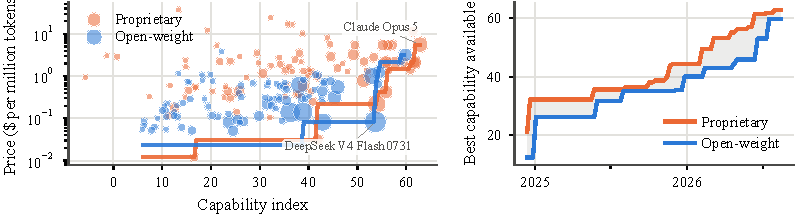
\includegraphics[width=\textwidth]{../figures/fig1_price_capability.pdf}
\caption{\textbf{The price of capability.} Left: posted blended price against the
capability index, with marker area proportional to the square root of token volume;
the step functions give the cheapest price available at or above each capability level
for each side of the market. Right: the highest capability available from each side by
release date, with the shaded region marking the open-weight lag.}
\label{fig:market}
\end{figure}

\subsection{Posted prices rarely move}

The archived catalogues let us follow the posted price of a model version from its
first appearance. Between consecutive captures, a median of three days apart, the
price changes \ChangeRate\% of the time. Over a model's observed life,
\NeverRepriced\% of models never change price at all. The left panel of
Figure~\ref{fig:prices} shows the survival of the launch price: \SurvSix\% of models
are still at their launch price after six months and \SurvTwelve\% after a year.
Conditional on a change, the median revision is a cut of about ten log points, and
\CutShare\% of changes are cuts.

Expressed the way the price-setting literature does, \MonthlyFreq\% of model-months
contain a price change, an expected duration of about \PriceDuration{} months. That is
at the low end of the range reported for consumer goods and comparable to online
retail \citep{bils2004,nakamura2008,cavallo2018}, which is itself the surprise: the
menu cost that explains rigidity in those settings, the physical and managerial cost of
changing a posted price, is close to zero when the price is a field in an API
catalogue. The distribution is also more polarised than in retail, where most goods are
repriced eventually. Here more than half of models are never repriced at all. What is
missing is not the ability to reprice but the incentive, which the next fact supplies.
The consequence for measurement is immediate: over the few weeks that a release event
study typically spans, an incumbent's posted price is unchanged with probability near
0.9, so a design that looks for the competitive effect of open weights in incumbent
price series is looking at a variable that rarely moves.

\subsection{Demand for a given model is price-inelastic in the short run}

We use the rare revisions to estimate how volume responds. Merging the archived
leaderboards with the archived catalogues gives \PanelObs{} model-date observations
on \PanelModels{} models between \PanelStart{} and \PanelEnd{}, containing
\NRevisions{} observations that follow a price change. We regress log volume on the
log fixed-weight price with model and date fixed effects, so identification comes
only from within-model revisions, net of anything common to the market on a date:
\begin{equation}
\log y_{jt} = \beta \log p_{jt} + \alpha_j + \gamma_t + \varepsilon_{jt}.
\label{eq:elasticity}
\end{equation}
Table~\ref{tab:elasticity} reports $\hat\beta$ = \ElastTok{} (s.e.\ \ElastTokSE) for
tokens and \ElastReq{} (s.e.\ \ElastReqSE) for requests. Open-weight and proprietary
models give indistinguishable estimates. Dropping the model fixed effects, so that
cross-model variation identifies $\beta$, moves the estimate to \ElastCross{}, which
is what one would expect if higher-priced models carry unobserved quality.

The right panel of Figure~\ref{fig:prices} traces the dynamics around \NPriceEvents{}
revisions, restricted to the captures that report non-overlapping weekly buckets so
that the path is not an artefact of a trailing aggregation window. Volume is flat
before the change and settles about 0.3 to 0.45 log points lower per log point of
price increase within a few weeks. The pre-period coefficients are small and
individually insignificant, which is the relevant check: if providers raised prices
after volume rose, the estimate would be biased toward zero, and we find no such
pattern.

An elasticity near one-half is not consistent with a static Bertrand equilibrium in
posted prices, which would require demand to be elastic at the optimum. We read it as
a short-run object. Switching a production workload to another model requires
re-testing prompts, harnesses and evaluation suites, so the relevant margin adjusts
over months rather than days. It also rationalises the rigidity: a provider that
would gain little volume from a price cut, and lose little from holding steady, has
weak incentive to reprice a model already in the field.

\begin{figure}[t]
\centering
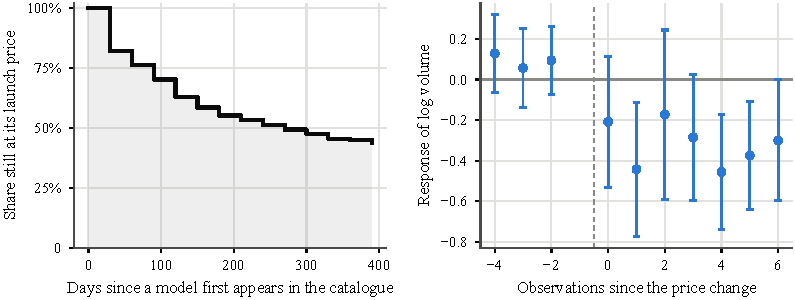
\includegraphics[width=\textwidth]{../figures/fig2_prices.pdf}
\caption{\textbf{Posted prices rarely move, and volume responds weakly when they do.} Left:
Kaplan-Meier survival of a model's launch price in the archived catalogues. Right:
coefficients from a distributed-lag version of \eqref{eq:elasticity} around
\NPriceEvents{} price revisions, scaled by the size of the revision, with model-by-event
and date fixed effects and 95\% intervals clustered by model.}
\label{fig:prices}
\end{figure}

\begin{table}[t]
\caption{Own-price elasticity of demand. Each column is a separate regression of
\eqref{eq:elasticity}. Standard errors clustered by model in parentheses.}
\label{tab:elasticity}
\centering
\small
\begin{tabular}{lccccc}
\toprule
& \multicolumn{2}{c}{Model and date FE} & \multicolumn{2}{c}{By openness} & Date FE only \\
\cmidrule(lr){2-3}\cmidrule(lr){4-5}\cmidrule(lr){6-6}
& Tokens & Requests & Open & Proprietary & Tokens \\
\midrule
$\log$ price & $-0.534$ & $-0.463$ & $-0.582$ & $-0.534$ & $-0.239$ \\
             & $(0.102)$ & $(0.087)$ & $(0.116)$ & $(0.204)$ & $(0.077)$ \\
\midrule
Observations & 19{,}803 & 19{,}803 & 8{,}873 & 10{,}930 & 19{,}803 \\
Models       & 634 & 634 & 321 & 316 & 634 \\
\bottomrule
\end{tabular}
\end{table}

\section{Entry without displacement}

The daily panel covers every model with usage for the four weeks to 20 August 2026, a
window containing \NEvents{} releases by providers with priced, scored models, of
which \NEventsOpen{} are open-weight. The window is unusual in one respect that turns
out to be the point: the market grew \MarketGrowth\% over it.

The left panel of Figure~\ref{fig:entry} decomposes daily volume into incumbents and
models released during the window. Entrants reached \EntrantShare\% of platform
tokens within four weeks, and \EntrantOpen\% of that volume went to open-weight
entrants.
Incumbent volume did not fall. It grew \IncumbentGrowth\%. Entry accounts for
\EntryGrowthShare\% of net growth, and the residual is incumbent expansion.

Aggregate volume can hide reallocation, so we test for it directly. For each release
$k$ at date $T_k$ we stack all incumbents $j$ that were already serving traffic, and
estimate
\begin{equation}
\log y_{jt} = \beta \, \mathbf{1}\{t \geq T_k\} \times \tau_{jk}
 + \delta_{jk} + \lambda_{kt} + X_{jt}'\theta + \varepsilon_{jkt},
\label{eq:diversion}
\end{equation}
where $\delta_{jk}$ is an incumbent-by-entrant effect and $\lambda_{kt}$ an
entrant-by-day effect, so that $\beta$ compares incumbents exposed to the same release
on the same day. The exposure measure $\tau_{jk} = S_{jk} \, r_{jk}$ combines
technological proximity with the entrant's relative value for money: $S_{jk} =
\exp(-\kappa d_{jk})$ with $d_{jk}$ the Mahalanobis distance between capability
vectors, and $r_{jk} = \log(q_k/p_k) - \log(q_j/p_j)$. Because capability and price
both trend, we also control for post-release interactions with the incumbent's own
capability and price.

We find no diversion. The estimate of $\beta$ is $0.01$ (s.e.\ $0.07$), and the
event-time path in the right panel of Figure~\ref{fig:entry} is flat on both sides of
the release. The confidence interval excludes differential declines larger than \DiversionMDE{}
log points per unit of exposure, and tightens to 0.10 and 0.04 under the Euclidean and
cosine distance measures reported in Table~\ref{tab:divrobust}. A design with ten releases over four weeks cannot detect small effects, and
we do not claim that diversion is zero. Nor can this design rule out that exposure is
measured with error: if capability similarity is a poor proxy for substitutability,
the null is uninformative about diversion even though it is informative about the
aggregate pattern. What we can say is that in a market growing at this rate, the
displacement channel is small relative to the expansion channel, which is the
comparison that matters for how the constraint operates.

\paragraph{A longer horizon.} Four weeks is short, and displacement plausibly takes
quarters. The archived panel lets us look further out. We take the \NMajor{}
open-weight releases in it that reached at least one percent of platform tokens, and
compare aggregate volume of models already in the market over the eight weekly
observations before and after each. Incumbent volume fell in \IncDeclineShare\% of
these episodes; the median change was $+\IncGrowthLong{}$ log points against a median
market change of $+\MktGrowthLong{}$. The release of DeepSeek R1 is the sharpest case:
platform volume rose 0.56 log points over the sixteen weeks around it while incumbent
volume was flat at $-0.03$. Incumbents lose share, because the market grows around
them, but for the most part they do not lose volume.

\begin{figure}[t]
\centering
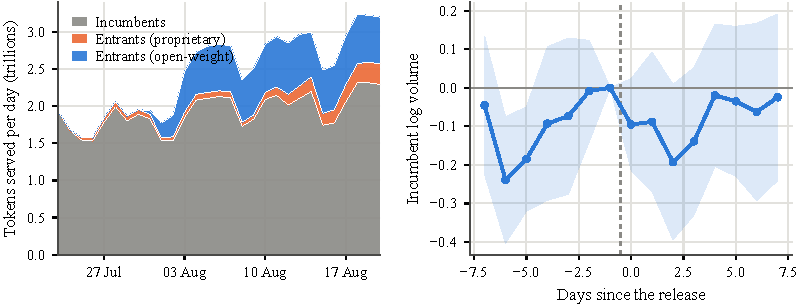
\includegraphics[width=\textwidth]{../figures/fig3_entry.pdf}
\caption{\textbf{Entry is absorbed by growth.} Left: daily platform volume split
between models already serving traffic at the start of the window and models released
during it. Right: event-time coefficients from \eqref{eq:diversion} on log incumbent
volume, per unit of exposure to the entrant, with 95\% intervals clustered by
incumbent.}
\label{fig:entry}
\end{figure}

\section{What open weights are worth}

Because posted prices do not respond and incumbents are not displaced, the value of
open-weight competition has to be measured on the choice set rather than on prices. We
estimate a nested-logit demand system over the \CFmodels{} models with prices and
capability scores, nesting models by capability tercile so that models of similar
capability are closer substitutes than models drawn from different tiers. Writing
$g(j)$ for the nest of model $j$ and $\sigma \in [0,1)$ for the within-nest
correlation \citep{cardell1997,berry1994}, shares take the form
\begin{equation}
s_j = \frac{\exp\!\big(\delta_j/(1-\sigma)\big)}{D_{g(j)}} \cdot
      \frac{D_{g(j)}^{\,1-\sigma}}{1 + \sum_h D_h^{\,1-\sigma}},
\qquad
D_g = \sum_{k \in g} \exp\!\big(\delta_k/(1-\sigma)\big),
\label{eq:shares}
\end{equation}
with mean utility $\delta_j = \beta_p \log p_j + \alpha' x_j + \xi_j$, where $x_j$
collects the capability index, context length, modality, reasoning support, latency
and age. The outside option is the fringe of models we cannot score, which holds
\CFoutside\% of tokens.

Two features of \eqref{eq:shares} make the exercise tractable. Observed shares invert
to mean utilities, $\delta_j = \log s_j - \log s_0 - \sigma \log s_{j \mid g(j)}$
\citep{berry1994}, so the system reproduces the data exactly and no part of the
counterfactual depends on how well the characteristics fit. And the counterfactual
depends only on $(\beta_p, \sigma)$: deleting the open-weight models from the choice
set changes the denominators in \eqref{eq:shares}, redistributing their volume across
the remaining models and the outside option.

\paragraph{Choosing the parameters.} We do not attempt to identify $\beta_p$ and
$\sigma$ from cross-sectional share variation, because the instruments this literature
relies on fail in this market. The differentiation instruments of \citet{gandhi2019}
are functions of the distribution of rival characteristics, which here is a
distribution over an essentially one-dimensional capability index, so they are
near-collinear with a model's own capability and therefore with its unobserved quality.
The obvious cost shifter, parameter count, is available only for open-weight models
and predicts unmeasured quality about as strongly as it predicts serving cost: in our
data it correlates 0.65 with the capability index, and instrumenting with it moves the
price coefficient from $-0.79$ under ordinary least squares to $-0.27$ despite a
first-stage $F$ above 900, which is the signature of a violated exclusion restriction
rather than of a corrected bias. We
therefore fix $\beta_p = -1$, between the within-model estimate of Section~3.3 and the
value near one reported by \citet{demirer2025}, and report every result across a range
of $\sigma$.

\paragraph{Results.} Removing open-weight models from the choice set at posted prices,
the average price paid per token rises from \$0.70 to \$1.80, an increase of
\CFprice\%. Consumer surplus, computed as the log-sum expected utility of
\citet{small1981}, falls \CFcs\%, worth about \$\CFdollars{}m per day at the platform's
current volume. The percentage change in surplus does not depend on $\beta_p$, which
enters the baseline and the counterfactual identically; only the conversion into
dollars scales with it. The loss is larger when substitution within a capability tier
is weaker, ranging from \$3.9m to \$1.3m per day as $\sigma$ moves from 0 to 0.7
(Figure~\ref{fig:cf} and Table~\ref{tab:cfgrid}). It also depends on how large the
outside option is taken to be, which is a modelling choice rather than a measurement:
raising the outside share from the observed 2.4\% to 50\% raises the proportional
surplus loss, from 21\% to 47\%, while lowering the dollar figure to \$1.0m per day.
The price effect is invariant to both. The price effect is almost invariant
to $\sigma$, because it is governed by the composition of the surviving choice set
rather than by the strength of substitution. Concentration moves against the
presumption that open weights fragment the market: the provider Herfindahl index rises
from \CFhhiBase{} to \CFhhiCf{} when open models are removed, because open-weight
volume is spread across more suppliers than the proprietary volume that replaces it.

These numbers hold prices fixed. That is the right convention given the rigidity
documented in Section~3.2, and it makes the exercise a statement about variety rather
than about pricing conduct, but it understates the long-run effect. Allowing
proprietary providers to reprice would require a pricing model, and the elasticity in
Section~3.3 is not consistent with the static Bertrand model that would ordinarily
supply one, so we leave that margin unpriced and read our estimates as a lower bound.

The left panel of Figure~\ref{fig:cf} repeats the exercise separately in each of the
\Ntasks{} task-level markets, where shares of spending are reported directly. The
implied price increase rises almost one for one with the open-weight share of task
spending, with a slope of 0.98. Averaged across tasks and weighted by spending, prices
rise \TaskCFprice\% and surplus falls \TaskCFcs\%, with the largest effects in agentic
and coding work, where open-weight models hold about a third of spending, and the
smallest in data extraction and transformation, where they hold under a sixth. The
task-level numbers are smaller than the aggregate because task shares are measured on
spending, which weights the expensive proprietary models that open weights do not
displace.

\begin{figure}[t]
\centering
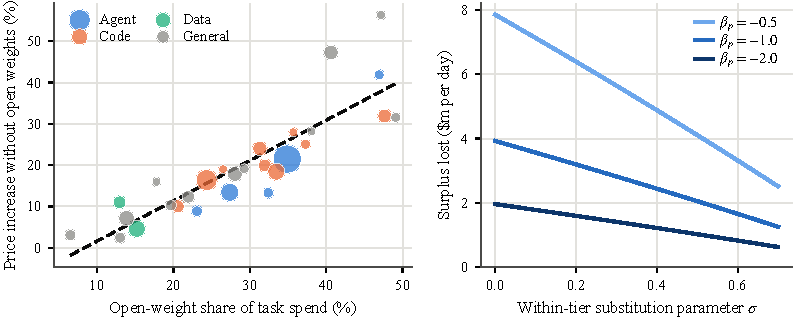
\includegraphics[width=\textwidth]{../figures/fig4_counterfactual.pdf}
\caption{\textbf{The value of the open-weight choice set.} Left: for each of the
\Ntasks{} task markets, the price increase implied by removing open-weight models
against their share of task spending; marker area is proportional to the task's share
of platform spending. Right: aggregate surplus loss per day across values of the
within-tier substitution parameter and the price coefficient.}
\label{fig:cf}
\end{figure}

\section{Discussion}

The three facts fit together. Short-run demand for a given model is inelastic, so
providers gain little by cutting the price of a model in the field and do not; because
posted prices do not move, competition is expressed in the terms on which new models
enter; and because the market is growing quickly, entrants can take a large share of
volume without taking it from anyone. In that environment, the standard empirical
signature of competitive discipline, a price response by incumbents, is absent even
though the constraint is economically large. Our counterfactual puts the value of the
open-weight choice set at roughly one fifth of consumer surplus on this platform.

\paragraph{A simple account.} The three fit together through the share of demand that
is actually in play. Let $M_t$ be total demand, growing at rate $g$ per period, and let
a fraction $\phi$ of existing demand be revisited each period, whether because a
workload is rebuilt or because a team re-evaluates its choice. Contestable demand is
$(g + \phi) M_t$, and a model's volume evolves as
\begin{equation}
y_{j,t+1} = (1 - \phi)\, y_{jt} + \sigma_j \,(g + \phi)\, M_t ,
\label{eq:accounting}
\end{equation}
where $\sigma_j$ is its share of contestable demand. Three implications follow.
An incumbent loses volume only when $\sigma_j (g+\phi) M_t < \phi\, y_{jt}$, that
is, when its share of contestable demand falls below $\phi/(g+\phi)$ times its
share of the stock; with $g \approx 0.13$ per week in our window, an incumbent with an
average share of new demand keeps growing. An entrant reaches a share of about
$\sigma_k (g+\phi)/(1+g)$ after one period, so entrants can take a large share of
volume quickly without anyone shrinking. And a permanent price change reaches only the
contestable margin, so the response measured $\tau$ periods out is attenuated by
roughly $1 - (1-\phi-g)^{\tau}$ relative to its long-run value.

That last point bounds how much of the inelasticity is an artefact of slow adjustment.
Taking $\phi + g \approx 0.23$ per week and the six weekly observations over which
Figure~\ref{fig:prices} shows the response settling, the attenuation factor is about
0.8, so the long-run elasticity implied by our estimate is near $-0.6$. Demand for a
given model is inelastic even after adjustment. The static first-order condition of a
provider maximising current profit is therefore not satisfied at the posted price,
which leaves two readings: providers price against a margin we do not observe, such as
capacity, hardware amortisation or the option value of usage; or the posted price is
not chosen to maximise current profit at all. The rigidity in Section~3.2 favours the
second.

This also reconciles two readings of the existing evidence. \citet{nagle2025} find
that a great deal of proprietary usage sits on models dominated by an open
alternative, and infer large foregone savings. That pattern is a puzzle if demand
adjusts quickly; it is what one should expect if the short-run elasticity is about
one-half and switching a workload is costly. The gains they identify are real, but
they accrue as workloads turn over rather than as incumbents reprice.

\paragraph{Limitations.} Our market is one router, and one that selects for
price-sensitive developers, so the elasticities and the counterfactual describe the
segment where substitution toward open weights is easiest. The capability index is
built from third-party benchmarks that compress into a single dimension, and models
that look identical on it are plainly not interchangeable in practice, which is
precisely why the discrete-choice approach is needed and also why the index should
not be read as a complete description of quality. We do not identify $\beta_p$ and
$\sigma$ from the data and instead report sensitivity across a range; a design with
exogenous variation in the choice set, such as a large release observed over a longer
window, would pin them down. The diversion test has power against moderate effects
only. Finally, the counterfactual holds prices fixed, and is therefore silent about
how the proprietary frontier would be priced in a world without open weights.

\paragraph{Implications.} For policy, the result reframes what to measure. Debates
about the competitive effect of open weights have proceeded on the presumption that
the effect, if real, would show up in the prices proprietary providers charge. In a
market where posted prices are set once and left alone, that presumption is wrong, and
an assessment based on incumbent price responses will conclude that open weights do
not matter. The relevant margin is the price at which the next unit of demand is
served, and on that margin the constraint is substantial.

\bibliographystyle{plainnat}
\begin{thebibliography}{99}

\bibitem[Bengio et al.(2026)]{bengio2026}
Y.~Bengio et al.
\newblock International AI Safety Report 2026.
\newblock arXiv:2602.21012, 2026.

\bibitem[Berry(1994)]{berry1994}
S.~Berry.
\newblock Estimating discrete-choice models of product differentiation.
\newblock {\em RAND Journal of Economics}, 25(2):242--262, 1994.

\bibitem[Berry et al.(1995)]{blp1995}
S.~Berry, J.~Levinsohn, and A.~Pakes.
\newblock Automobile prices in market equilibrium.
\newblock {\em Econometrica}, 63(4):841--890, 1995.

\bibitem[Bils and Klenow(2004)]{bils2004}
M.~Bils and P.~J. Klenow.
\newblock Some evidence on the importance of sticky prices.
\newblock {\em Journal of Political Economy}, 112(5):947--985, 2004.

\bibitem[Cardell(1997)]{cardell1997}
N.~S. Cardell.
\newblock Variance components structures for the extreme-value and logistic
  distributions with application to models of heterogeneity.
\newblock {\em Econometric Theory}, 13(2):185--213, 1997.

\bibitem[Cavallo(2018)]{cavallo2018}
A.~Cavallo.
\newblock Scraped data and sticky prices.
\newblock {\em Review of Economics and Statistics}, 100(1):105--119, 2018.

\bibitem[Demirer et al.(2025)]{demirer2025}
M.~Demirer, A.~Fradkin, N.~Tadelis, and S.~Peng.
\newblock The emerging market for intelligence: Pricing, supply, and demand for LLMs.
\newblock NBER Working Paper 34608, 2025.

\bibitem[Gandhi and Houde(2019)]{gandhi2019}
A.~Gandhi and J.-F. Houde.
\newblock Measuring substitution patterns in differentiated-products industries.
\newblock NBER Working Paper 26375, 2019.

\bibitem[Korinek and Vipra(2025)]{korinek2025}
A.~Korinek and J.~Vipra.
\newblock Concentrating intelligence: Scaling and market structure in artificial
  intelligence.
\newblock {\em Economic Policy}, 40(121):225--256, 2025.

\bibitem[Nagle and Yue(2025)]{nagle2025}
F.~Nagle and D.~Yue.
\newblock The latent role of open models in the AI economy.
\newblock Working paper, 2025.

\bibitem[Nakamura and Steinsson(2008)]{nakamura2008}
E.~Nakamura and J.~Steinsson.
\newblock Five facts about prices: A reevaluation of menu cost models.
\newblock {\em Quarterly Journal of Economics}, 123(4):1415--1464, 2008.

\bibitem[Nevo(2001)]{nevo2001}
A.~Nevo.
\newblock Measuring market power in the ready-to-eat cereal industry.
\newblock {\em Econometrica}, 69(2):307--342, 2001.

\bibitem[Small and Rosen(1981)]{small1981}
K.~A. Small and H.~S. Rosen.
\newblock Applied welfare economics with discrete choice models.
\newblock {\em Econometrica}, 49(1):105--130, 1981.

\end{thebibliography}

\appendix

\section{Data construction}
\label{app:data}

\paragraph{Endpoints.} The catalogue endpoint returns, for every listed model, the
posted input and output price per token, context length, input and output modalities,
a creation timestamp, and the Hugging Face repository identifier when the weights are
public. The leaderboard endpoint returns tokens, requests, tool calls and media counts
by model and serving variant. A benchmark endpoint returns third-party capability
scores and usage-weighted effective prices. A task endpoint returns, for each of
\Ntasks{} usage categories, the category's share of platform spending and the share
held by each of its ten largest models, in both spending and token terms. An endpoint
listing gives each hosting provider's price, quantisation and uptime for a given
model. All are public and unauthenticated.

\paragraph{Daily usage.} Each model's public page embeds its own trailing-month daily
usage series in the page's streamed render payload. We request one page per model with
observed usage and parse the payload, which yields \Nactive{} models over 30 days. The
same payload carries per-endpoint latency and throughput percentiles, which we
aggregate to the model level by request count.

\paragraph{Historical coverage.} Internet Archive captures supply history. Captures of
the catalogue endpoint give a price and characteristic panel from July 2023. Captures
of the leaderboard page embed the leaderboard payload in the same streamed format, so
we recover model-level usage without relying on the rendered page. Two vintages are
present and we treat them separately: captures before late 2024 embed a series of
non-overlapping weekly buckets, and later captures embed a single trailing-window
snapshot. Shares are comparable across vintages; levels are not, so all specifications
include date fixed effects, and Table~\ref{tab:robust} reports the two vintages
separately. We fetch captures at a fixed spacing with adaptive backoff, which is the
binding cost of the collection: the archive requests take a few hours, and every other
step runs in minutes on a laptop.

\paragraph{Merging.} Usage and price observations are matched by model identifier and
nearest date within ten days. Openness is taken from the current catalogue where the
model is still listed, because the weight-repository field is absent from the earliest
captures. Prices are dollars per million tokens throughout. The fixed-weight price
index used in \eqref{eq:elasticity} weights posted input and output prices by the
sample-mean token mix, so that it carries no feedback from a model's own usage
composition; Table~\ref{tab:robust} shows the estimate is not sensitive to that choice.

\section{Capability imputation}

Benchmark scores are missing for smaller models. For each missing dimension we fit a
ridge regression on the dimensions the model does have, using models scored on both,
and predict the missing value. Masking half of the fully scored models and predicting
the held-out values gives $R^2$ of 0.99, 0.97 and 0.96 for the reasoning, coding and
agentic dimensions, with mean absolute errors of 1.7, 5.0 and 3.1 points against
standard deviations of 16.4, 22.6 and 18.5. Imputation raises coverage from 109 models
and 77\% of tokens to \Nscored{} models and \CovScored\% of tokens. All results in the
main text hold on the directly scored subsample.

\section{Robustness}

Table~\ref{tab:robust} reports the elasticity across price measures, outcome measures,
capture vintages, openness and sample period. The estimate stays between $-0.38$ and
$-0.63$. The realised blended price, which mixes posted prices with the model's own
input-output composition, gives the largest magnitude, as expected if a shift toward
prompt-heavy workloads lowers the average price per token and raises volume at the
same time; the fixed-weight index removes that channel and is our preferred measure.

Two further checks bear on the elasticity. A price cut may accompany the launch of a
replacement by the same provider, which would depress the old model's volume for
reasons other than price. Adding an indicator for observations within 28 days of a
same-provider release, which covers 38\% of the panel, leaves the estimate at
$-0.534$; dropping those observations gives $-0.499$ (s.e.\ 0.123).

Table~\ref{tab:divrobust} reports the diversion test under three definitions of
technological distance. None of the six estimates is distinguishable from zero. The
Euclidean and cosine measures give tighter standard errors than the Mahalanobis
measure, and bound the differential decline for the most exposed incumbents at 0.13
and 0.09 log points respectively.

\begin{table}[h]
\caption{Own-price elasticity across specifications. Each row is a separate estimate of
\eqref{eq:elasticity} with model and date fixed effects; standard errors clustered by
model.}
\label{tab:robust}
\centering
\small
\begin{tabular}{lrrrr}
\toprule
Specification & Estimate & Std.\ error & Observations & Models \\
\midrule
Fixed-weight price (baseline) & $-0.534$ & 0.102 & 19{,}803 & 634 \\
Input price                   & $-0.526$ & 0.096 & 19{,}803 & 634 \\
Output price                  & $-0.485$ & 0.109 & 19{,}803 & 634 \\
Realised blended price        & $-0.658$ & 0.095 & 19{,}803 & 634 \\
Requests rather than tokens   & $-0.463$ & 0.087 & 19{,}803 & 634 \\
Weekly captures only          & $-0.472$ & 0.123 & 15{,}133 & 432 \\
Trailing captures only        & $-0.476$ & 0.125 & 4{,}670 & 428 \\
Open-weight models            & $-0.582$ & 0.116 & 8{,}873 & 321 \\
Proprietary models            & $-0.534$ & 0.204 & 10{,}930 & 316 \\
2025 onwards                  & $-0.527$ & 0.100 & 7{,}906 & 542 \\
\bottomrule
\end{tabular}
\end{table}

\begin{table}[h]
\caption{Diversion at entry under alternative distance measures. Each row estimates
\eqref{eq:diversion} with incumbent-by-entrant and entrant-by-day fixed effects and
post-release controls for the incumbent's own capability and price.}
\label{tab:divrobust}
\centering
\small
\begin{tabular}{llrrr}
\toprule
Distance & Exposure & Estimate & Std.\ error & Observations \\
\midrule
Mahalanobis & similarity $\times$ relative value & $0.010$ & 0.070 & 11{,}820 \\
Mahalanobis & similarity                         & $0.019$ & 0.120 & 11{,}820 \\
Euclidean   & similarity $\times$ relative value & $-0.006$ & 0.047 & 11{,}820 \\
Euclidean   & similarity                         & $0.008$ & 0.065 & 11{,}820 \\
Cosine      & similarity $\times$ relative value & $0.022$ & 0.031 & 11{,}820 \\
Cosine      & similarity                         & $0.083$ & 0.086 & 11{,}820 \\
\bottomrule
\end{tabular}
\end{table}

\section{Counterfactual sensitivity}

Table~\ref{tab:cfgrid} reports the counterfactual across the within-tier substitution
parameter, and \texttt{robustness.json} reports it across the size of the outside
option as well. The price effect is nearly invariant to $\sigma$, because it is driven by
the composition of the surviving choice set rather than by the strength of
substitution. The surplus loss falls as $\sigma$ rises, because closer substitutes
within a capability tier make the proprietary models better replacements for the
open-weight models that leave.

\begin{table}[h]
\caption{The open-weight counterfactual across substitution parameters, at
$\beta_p = -1$. Prices are dollars per million tokens; the surplus loss is evaluated at
the platform's volume on the reference day.}
\label{tab:cfgrid}
\centering
\small
\begin{tabular}{lrrrrr}
\toprule
$\sigma$ & Price paid & Price without open & Surplus change & Surplus loss & HHI \\
         & (\$/M)     & (\$/M)             & (\%)           & (\$m per day) & (without open) \\
\midrule
0.0 & 0.70 & 1.82 & $-33.8$ & 3.9 & 1109 \\
0.2 & 0.70 & 1.81 & $-27.5$ & 3.2 & 1082 \\
0.4 & 0.70 & 1.80 & $-21.0$ & 2.4 & 1048 \\
0.6 & 0.70 & 1.79 & $-14.3$ & 1.7 & 1006 \\
0.7 & 0.70 & 1.78 & $-10.8$ & 1.3 & \phantom{0}982 \\
\bottomrule
\end{tabular}
\end{table}

\newpage
\input{checklist}

\end{document}
